\section{Experimental Design and Methodology}\label{sec:exp}
This section describes the negotiation protocol, the nine benchmarked policies, the dual-simulator testbed, and the experimental design behind RQ1--RQ4.

\subsection{Decentralized Negotiation Protocol and Safeguards}\label{sec:proto}
All communicating policies run inside one five-mode agent state machine (\texttt{CRUISE}, \texttt{NEGOTIATE}, \texttt{YIELD}, \texttt{PROCEED}, \texttt{DONE}) stepped at $20$\,Hz (Supplementary Fig.~S7).



\emph{Conflict detection and snapshot resolution.} In \texttt{CRUISE}, robots broadcast 5\,Hz \texttt{STATE} beacons (pose, velocity, mode, corridor entry time), each considered fresh for 1.0\,s after receipt. A conflict starts when a peer beacon shows an opposing robot within $R_{\mathrm{det}} = 6.0$\,m, beyond the 3.5\,m Lidar range, so that negotiation begins before either robot passes a usable refuge. Each robot then freezes its state into a \texttt{Snapshot} $S_i$ (pose, speed bounds, urgency, payload) and resends it in a \texttt{BID} every $0.3$\,s. Every policy is a deterministic function of the sorted snapshot pair $(S_A, S_B)$ and the shared map, so both robots compute the same (yielder, proceeder, refuge) without a further handshake.

\emph{Lossy-channel safeguards and fallbacks.} Three switchable safeguards guard against decisions computed from different snapshots: \texttt{commit} attaches the planned decision to each \texttt{BID} and waits for mutual confirmation (the lower-ID robot's choice wins a disagreement; unconfirmed decisions expire after 3.0\,s); \texttt{state\_guard} makes a yielder abort to \texttt{PROCEED} if the peer's \texttt{STATE} shows it is also yielding or heading for the same bay; and \texttt{bay\_check} treats bays with Lidar returns within 0.45\,m of the parking spot as occupied. A proceeder advances only once \texttt{STATE} or Lidar confirms that the yielder is off-lane, and a parked yielder exits once \texttt{STATE} confirms passage, or, if \texttt{STATE} is stale, when Lidar confirms the peer has passed or after a random $U[6,12]$\,s hold with a clear lane. For liveness, robots fall back to reactive backoff when no peer \texttt{BID} arrives within $\tau_{\mathrm{neg}} = 3.0$\,s, a proceeder stalls for $\tau_{\mathrm{proc}} = 60.0$\,s, or no refuge is feasible ($\mathcal{F}=\emptyset$, 10.0\,s backoff); a valid peer \texttt{BID} resumes negotiation.

\emph{Map and multi-robot extensions.} \texttt{share\_map} attaches known bay IDs to every \texttt{BID}; \texttt{explore} starts robots knowing only the end rooms and adds bays seen by Lidar within 3.5\,m, optionally gating map exchange on Lidar peer detection (\texttt{share\_on\_detect}) or delaying the decision up to 15.0\,s for peer maps (\texttt{hold\_for\_map}); and \texttt{refuge\_blocked} cross-checks Lidar returns in a bay against peer \texttt{STATE}, broadcasting unmapped obstacles as blocked bays. For three robots, \texttt{make\_room} sends a follower that blocks its reversing leader into an upstream bay, and \texttt{goal\_wait} parks a robot whose branch destination is occupied in an upstream bay instead of the main lane.

\subsection{Evaluated Coordination Policies}\label{sec:pol}
Table~\ref{tab:taxonomy} summarizes the nine policies evaluated across the benchmark studies. All negotiating policies map the frozen snapshot pair $(S_A, S_B)$ to a yielder $Y \in \{A, B\}$ and feasible refuge $r \in \mathcal{F}(Y, P)$.

\subsubsection{Non-Communicating, Lock, and Heuristic Rulebook Policies}
\texttt{reactive} (R) uses no communication: when Lidar detects an oncoming peer within braking distance, the robot stops, waits a random patience $U[2,6]$\,s, and reverses into the nearest refuge behind it if the peer is still there. \texttt{backoff} (B) doubles the upper bound of the patience interval after each earlier yield, $U[0, 6\cdot2^{\min(k,5)}]$\,s.
\texttt{reservation} (S) emulates first-come, first-served zone control~\cite{fanti2002event}: a robot outside the corridor waits in its staging room while an opposing robot is inside (\texttt{rules\_default} breaks simultaneous entries). \texttt{fixed\_priority} (F), a prioritized-planning social law~\cite{cap2015prioritized}, makes the higher-ID robot yield into its best feasible refuge $r^\ast$.
\texttt{rules\_default} (D) is a rulebook in the sense of~\cite{censi2019rulebooks}: six tiers inspired by traffic etiquette~\cite{kato1992coordinating,highwaycode} and checked in order, namely (1)~the only robot with a feasible refuge yields; (2)~the less urgent robot yields if $|u_A - u_B| \ge 0.5$; (3)~an unloaded robot yields to a loaded one; (4)~the later corridor entrant (by $\ge 1.0$\,s) yields; (5)~the only robot with a refuge within 2.0\,m behind it yields; and (6)~the lower ID wins.
\texttt{rules\_proximity} (P) modifies this hierarchy by prioritizing geometry ahead of seniority, such that whichever robot is closer to its feasible refuge (by $\ge 0.1$\,m) yields immediately after checking payload. All rulebook thresholds were fixed from the Waffle specification and the etiquette sources before any benchmark run, and no policy parameter was tuned on benchmark outcomes; the only selected parameter is the fairness weight $\lambda$, chosen on separate sequences (Sec.~\ref{sec:rq2}). Their one-at-a-time sensitivity is reported in study \texttt{S11a}.

\begin{table*}[!t]\centering
\caption{Taxonomy of benchmarked corridor coordination policies across communication, information inputs, model assumptions, and strategic properties.}
\label{tab:taxonomy}
{\footnotesize\setlength{\tabcolsep}{2.9pt}
\begin{tabular}{@{}llcccc>{\raggedright\arraybackslash}p{0.190\textwidth}@{}}\toprule
Policy (Code) & Family & Comms & State Inputs Used & Motion Model & Incentive Prop. & Multi-Robot / Map Scope \\\midrule
\texttt{reactive} (R) & Local sensor backoff & None & $3.5$\,m Lidar proximity & None & N/A & Pairwise/local; patience $U[2,6]$\,s \\
\texttt{reservation} (S) & Corridor mutex lock & \texttt{STATE} & Occupancy, $t_{\mathrm{enter}}$ & None & First-in wins & Corridor FCFS; rulebook inside-tie \\
\texttt{fixed\_priority} (F) & Static social law & \texttt{STATE}+\texttt{BID} & Robot ID, feasibility & Feasibility only & Non-manipulable$^\dagger$ & Pairwise + \texttt{make\_room} / \texttt{goal\_wait} \\
\texttt{rules\_default} (D) & Lexicographic rules & \texttt{STATE}+\texttt{BID} & $u_i$, load, $t_{\mathrm{enter}}$, bay $\le 2$\,m & Feasibility only & Non-manipulable$^\dagger$ & Ordered 6-rule industrial etiquette \\
\texttt{rules\_proximity} (P) & Geometric rulebook & \texttt{STATE}+\texttt{BID} & Nearest-bay $|x_r - x_i|$, D & Refuge distance & Pose-dependent & Closest-refuge ahead of seniority \\
\texttt{learned} (L) & Tabular classifier & \texttt{STATE}+\texttt{BID} & Binned bay dist., $u_i$, load & Offline sim table & Co-op assumed & 93 states; unseen $\to$ fixed priority \\
\cb\ (C) & Kinematic auction & \texttt{STATE}+\texttt{BID} & Full \texttt{Snapshot}, $u_i$ & Constant-speed & Manipulable & Pairwise social-cost minimization \\
\gb\ (G) & Convoy auction & \texttt{STATE}+\texttt{BID} & Group \texttt{Snapshot}s & Side-level sum & Co-op assumed & Distinct bays across convoy group \\
\texttt{clarke} (V) & VCG mechanism & \texttt{STATE}+\texttt{BID} & Cost vectors $b_i(o)$ & Constant-speed & DSIC (unilat.)$^\ddagger$ & Externality payment to fleet bank \\\bottomrule
\end{tabular}}\\[2pt]
{\footnotesize $^\dagger$Non-manipulable with respect to cost bids; physical state claims ($u_i$, load, known bays) are assumed authentic. $^\ddagger$Dominant-strategy incentive compatible for unilateral cost scaling under the shared kinematic model; runs a budget surplus and does not prevent joint shading or bay-set omission.}
\end{table*}

\subsubsection{Kinematic Cost Bidding (\cb) and Convoy Group Bidding (\gb)}
Under \cb\ (C), robots choose the yielder that minimizes predicted urgency-weighted delay from Eq.~\eqref{eq:timeline}:

\begin{equation}
\begin{aligned}
\tilde{c}_Y &= \bigl(u_Y d_Y(r^\ast) + u_P d_P(r^\ast)\bigr)\exp(\sigma \epsilon_Y), \\
Y^\ast &= \arg\min_{Y\in\{A,B\}} \tilde{c}_Y,
\end{aligned}
\label{eq:costbid}
\end{equation}

where $\epsilon_Y \sim \mathcal{N}(0,1)$ adds log-normal estimation noise ($\sigma = 0$ unless stated) and $\tilde{c}_Y = \infty$ if no refuge is feasible. For convoys (yielding group $\mathcal{G}_Y$, proceeding group $\mathcal{G}_P$), \gb\ (G) attaches follower snapshots to the leader's \texttt{BID}, assigns distinct bays greedily to yielding members, and computes a side-level cost

\begin{equation}
\begin{aligned}
C_{\mathrm{grp}}(\mathcal{G}_Y,\mathcal{G}_P) &= \sum_{y\in\mathcal{G}_Y} u_y d_y(r_y^\ast) \\
&\quad + \Bigl(\max_{f\in\mathcal{G}_P\setminus\{P\}}\frac{|x_f-x_P|}{v_{\max,f}}\Bigr)\!\sum_{y\in\mathcal{G}_Y} u_y \\
&\quad + \Bigl(\max_{y\in\mathcal{G}_Y} d_{P,y}(r_y^\ast)\Bigr)\!\sum_{p\in\mathcal{G}_P} u_p.
\end{aligned}
\label{eq:groupbid}
\end{equation}

whose terms are the yielding group's delays, its wait while proceeding followers pass, and the proceeding group's wait while the slowest yielder parks. Summing member delays assumes concurrent maneuvers and ignores the \emph{serial} wait while followers reverse via \texttt{make\_room}.

\subsubsection{Clarke-Pivot (VCG) Mechanism and Repeated Fairness Credit}
Because robots can inflate bids to avoid yielding, \texttt{clarke} (V) implements the Vickrey--Clarke--Groves pivot mechanism~\cite{clarke1971multipart}: each robot reports its delay cost $b_i(o)$ for both outcomes $o \in \{A, B\}$ ($o$ names the yielder), and the mechanism selects the cost-minimizing $o^\ast$ and charges each robot an externality payment $p_i$ into an operator ledger,
\begin{equation}
\begin{aligned}
o^\ast &= \arg\min_{o\in\{A,B\}} \sum_{i\in\{A,B\}} b_i(o), \\
p_i &= \sum_{j\neq i} b_j(o^\ast) - \min_{o\in\{A,B\}} \sum_{j\neq i} b_j(o) \ge 0.
\end{aligned}
\label{eq:clarke}
\end{equation}
Because each robot pays the exact delay penalty it imposes on the other, truthful reporting ($b_i(o) = u_i d_i(r^\ast(o))$) is a dominant strategy in any single encounter.
In cooperative fleets with repeated encounters ($t = 1, \dots, K$), strictly minimizing single-shot delay can repeatedly burden the same robot. To maintain long-run equity without monetary transfers, this study evaluates a karma-inspired~\cite{censi2019karma,elokda2024karma} credit rule governed by a fairness weight $\lambda \ge 0$ via
\begin{equation}
\begin{aligned}
o_t^\ast &= \arg\min_{o\in\{A,B\}} \Bigl[d_{A,t}(o)+d_{B,t}(o) \\
&\quad + \lambda\bigl(D_{o,t-1}^{\mathrm{cum}} - D_{\bar{o},t-1}^{\mathrm{cum}}\bigr)\Bigr], 
\end{aligned}
\label{eq:karma}
\end{equation}
where $o$ denotes the yielding robot, $\bar{o}$ the other robot, and $D_{i,t-1}^{\mathrm{cum}}$ robot $i$'s cumulative delay over the previous $t-1$ encounters. Setting $\lambda = 0$ gives pure social-cost minimization, while $\lambda > 0$ makes it costlier to choose as yielder the robot that has already accumulated more delay. We also evaluate the balance form that penalizes the post-encounter gap, $\lambda\,|(D_{A,t-1}^{\mathrm{cum}}+d_{A,t}(o))-(D_{B,t-1}^{\mathrm{cum}}+d_{B,t}(o))|$. For both forms, $\lambda$ is selected on 50 sequences and reported on 100 fresh sequences, with exact or log-normally perturbed delay estimates $d$.

\subsubsection{Tabular Outcome Classifier (\texttt{learned}, L)}
\texttt{learned} keys each conflict on binned distances to the nearest feasible refuge behind each robot, the sign of $u_A-u_B$, and both payload flags. It is trained on 800 two-bay encounters by simulating both forced outcomes (full information, 93 keys), picks the outcome with the lower mean weighted delay, and falls back to \texttt{fixed\_priority} on unseen keys (details in Supplementary Sec.~S-II).


\subsubsection{Dual-Simulator Testbed}
The same 20\,Hz Python \texttt{Agent} class runs in two environments. The 2D unicycle simulator \texttt{sim2d} integrates motion at 20\,Hz under linear and angular acceleration limits, models peers as unoccluded $0.25$\,m circles within 3.5\,m, and checks footprint collisions at every step with the Separating Axis Theorem (SAT); at $>500\times$ real time it executes the 18 original studies ($50{,}714$ episodes) and the 8 revision studies ($72{,}310$ episodes). Bid noise is seeded per robot from the episode seed and the decision time \texttt{round(t,1)}, so the robots share a draw only when their snapshots carry identical timestamps; the revision studies also key noise per episode (seed and robot), which also pairs Gazebo noisy-bid runs exactly ($12/12$ same first yielder). The 3D stack compiles each scenario into a Gazebo Harmonic world with TurtleBot3 Waffles and $360^\circ$ \texttt{LaserScan} sensors~\cite{turtlebot3,gazebosim}. Each robot runs an \texttt{agent\_node} that reads ground-truth pose (isolating negotiation from SLAM drift), filters static wall returns and clusters the remaining points ($0.35$\,m linkage) into peer positions, and exchanges JSON packets over a bus with emulated latency, jitter, and loss; a \texttt{referee\_node} logs the same metrics and SAT collision checks as \texttt{sim2d}.

\subsection{Scenario Topologies and Experimental Matrix}
Default physical, kinematic, and protocol parameters are listed in Supplementary Table~S-II. In the base two-robot encounter (Fig.~\ref{fig:scen}a,b), Robot~$A$ starts at $x = -1.0$\,m ($t = 0$) heading eastbound toward its goal at $x = L + 2.0$\,m, while Robot~$B$ starts at $x = L + 1.0$\,m heading westbound toward $x = -2.0$\,m after a random delay drawn from $U[0, 8]$\,s (or $U[0, 10]$\,s in 10\,m corridors). Because Robot~$A$ requires $\approx 35$\,s to traverse the corridor while Robot~$B$ enters within $\approx 12$\,s, every random draw produces a genuine head-on conflict inside the aisle, with the meeting point varying relative to the bays.

The benchmark spans six scenarios over five geometries: the single-bay and two-bay corridors, the heterogeneous-fleet corridor (differing urgency, speed, and payload), a 2-vs.-1 convoy in which follower $C$ trails leader $A$ by 1.2\,m against oncoming $B$ (Fig.~\ref{fig:scen}c), and a T-junction with a 2.0\,m-deep side branch at $x = 5.5$\,m, run as branch exit and branch turn-in (Fig.~\ref{fig:scen}d).
\begin{figure*}[!t]
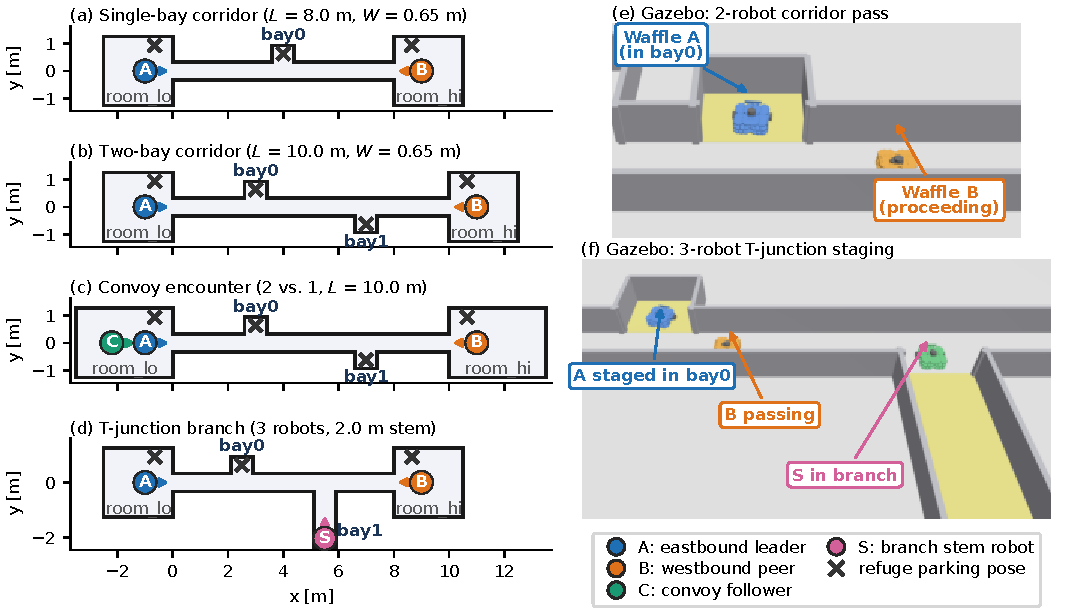
\includegraphics[width=1\textwidth]{Images/scenarios.pdf}
\caption{Benchmark scenario topologies and 3D validation environment. (a)--(d) Top-down 2D layouts (light gray: navigable space; $\times$: discrete refuge parking positions; colored discs/arrows: initial robot poses and travel directions). In (d), the turn-in variant is shown where robot~$S$ starts parked in the branch stem (\texttt{bay1}) and robot~$A$'s destination is \texttt{bay1}; in the exit variant, $A$ and $B$ traverse end-to-end while $S$ exits \texttt{bay1}. (e)--(f) Gazebo Harmonic renders ($3840\times2160$ camera): (e) Waffle~$A$ parked in \texttt{bay0} while $B$ passes; (f) T-junction turn-in with $A$ staged in \texttt{bay0} under \texttt{goal\_wait}, $B$ passing, and $S$ leaving the branch.}
\label{fig:scen}
\end{figure*}
Table~\ref{tab:design} details the experimental design across RQ1--RQ4: 18 original 2D studies ($50{,}714$ episodes), 8 revision studies ($72{,}310$ episodes), and 496 seed-paired ROS~2 / Gazebo Harmonic runs (460 main runs plus 36 hold-mode runs). The encounter distribution of each study is uniform over its grid cells, with $B$'s start delay drawn from $U[0,8]$\,s ($U[0,10]$\,s in 10\,m corridors); seeds within a cell are the replicates, and every policy sees the same draws.

\begin{table*}[!t]\centering
\caption{Experimental design grouped by research question. Parameters follow Supplementary Table~S-II unless stated. $N$ counts executed episodes; each hindsight reference executes two forced runs per draw. Study S5 was retired before release; labels match the released data files.}
\label{tab:design}
{\footnotesize\setlength{\tabcolsep}{3.4pt}
\begin{tabular}{@{}ll>{\raggedright\arraybackslash}p{0.35\textwidth}rlr@{}}\toprule
Layer / RQ & Study (Sec.) & Factorial Grid Factors & Seeds & Policies Evaluated & $N$ \\\midrule
\multirow{6}{*}{RQ1 (Sec.~\ref{sec:rq1})}
 & Single bay (\texttt{S1}) & Bay $x\in\{1,2,3,4,5,6,7\}$\,m & 60 & R, F, D, P, C, O, O$_w$ & 2,940 \\
 & Zone reservation & Bay $x\in\{1,\dots,7\}$\,m (separate 30-seed draw set) & 30 & S, F, D, C, forced A/B & 1,260 \\
 & Two bays (\texttt{S4}) & Bay 1 $\{2,3,4\}\times$ Bay 2 $\{6,7,8\}$\,m $\times$ side; B $U[0,10]$\,s & 20 & R, F, D, P, C, O, O$_w$ & 2,520 \\
 & Asymmetric robots (\texttt{S2}) & $u_B\in\{1,3\}\times$ load $\{0,1\}\times v_B\in\{0.26,0.13\}$\,m/s $\times$ bay $\{2,4,6\}$\,m & 30 & R, F, D, P, C, O, O$_w$ & 5,040 \\
 & Noisy bids (\texttt{S7}) & $\sigma\in\{0,0.1,0.25,0.5,1.0\}\times$ bay $x\in\{1,\dots,7\}$\,m & 30 & C, P, O & 1,470$^\ast$ \\
 & Learned classifier & Train: 800 two-bay pairs; Eval: 150 ID + 150 OOD & -- & L, F, D, C, O$_w$ & 1,600+1,500 \\\midrule
\multirow{3}{*}{RQ2 (Sec.~\ref{sec:rq2})}
 & Unpriced misreport (\texttt{S6}) & B bid scale $k\in\{1,1.5,2,4,10\}\times$ bay $x\in\{2,4,6\}$\,m & 60 & C, O & 1,080 \\
 & Clarke VCG (\texttt{S9}) & Deviator $\{\text{A, B, AB}\}\times 10$ scales $k\in[0.25,4]\times u_B\{1,3\}\times$ bay $\{2,4,6\}$ & 60 & V (+ none/naive eval) & 10,080 \\
 & Repeated fairness (\texttt{S10}) & 50 sequences $\times$ 20 encounters, bay $U[1,7]$\,m; $\lambda\in\{0,0.25,0.5,1,2\}$ & -- & forced A/B (offline) & 2,000 \\\midrule
\multirow{7}{*}{RQ3 (Sec.~\ref{sec:rq3})}
 & Comms sweep (\texttt{S3}) & Loss $\{0,10,30,50,70,90\}\%\times\tau\in\{0.05,0.25,0.5,1,2\}$\,s & 30 & F, D, P, C & 3,600 \\
 & Comms stress (\texttt{S8}) & $R_{\mathrm{det}}\{6,3,1.5\}$\,m $\times v\{0.26,0.5\}$\,m/s $\times$ loss $\{0,50,90\}\%\times\tau\{0.05,0.5,2\}$\,s & 20 & F, D, P, C & 4,320 \\
 & Extreme comms (\texttt{S8b}) & $R_{\mathrm{det}}\in\{1.5,6\}$\,m $\times$ loss $\{90,97,99\}\%\times\tau\in\{2,4,8\}$\,s; $v=0.5$\,m/s & 20 & F, D, P, C & 1,440 \\
 & Safeguard ablation (\texttt{S8c}) & \texttt{S8b} grid $\times$ \texttt{commit} $\{0,1\}\times$ \texttt{state\_guard} $\{0,1\}\times$ \texttt{bay\_check} $\{0,1\}$ & 20 & F, C & 5,760 \\
 & Asymmetric maps & 7 bay-knowledge splits $\times$ \texttt{share\_map} $\{0,1\}\times$ loss $\{0,50\}\%$; bays $3,7$\,m & 10 & F, D, C & 840 \\
 & Blocked bays & Physically obstructed bays $\in\{\emptyset,\text{bay0},\text{bay1},\text{both}\}\times$ loss $\{0,50\}\%$ & 10 & R, F, D, C & 320 \\
 & Explore \& hold & 4 map modes $\times R_{\mathrm{det}}\in\{6,3.5\}$\,m $\times$ loss $\{0,50\}\%$ (+ hold batch) & 30 & F, D, C & 1,440+360 \\\midrule
\multirow{3}{*}{RQ4 (Sec.~\ref{sec:rq4})}
 & Convoy 2 vs.\ 1 & B type (equal, loaded, $u_B=3$) $\times$ bays $\{2,4\}\times\{6,8\}\times$ delay $\{0,4,8\}\times$ loss & 3 & F, D, C, G, side ref. & 1,080 \\
 & T-junction (3 robots) & Delays $(A,B,S)\in\{0,4\}\times\{0,4,8\}\times\{0,6\}$\,s $\times 2$ S goals $\times$ loss $\{0,50\}\%$ & 2 & R, F, D, C & 384 \\
 & ROS~2 / Gazebo 3D & Seed-paired reduced grid across all studies + 36 hold runs & 6--10 & R, S, F, D, P, L, C, G, V, O & 460+36 \\\midrule
\multirow{6}{*}{Revision}
 & Dense noise (\texttt{S7d/h}) & 10 $\sigma$ levels $\times$ noise keying; \texttt{S1}, \texttt{S2} grids & 30 & C, P, D, F, O, O$_w$ & 18,390 \\
 & Planner error (\texttt{S7m}) & $v_{\mathrm{rev}},\omega_{\max}$ error $\pm10$--$30\%$; \texttt{S1}, \texttt{S2} & 30 & C, P, D, F, O & 16,740 \\
 & Correlated loss (\texttt{S8d}) & i.i.d./burst/blackout, fresh seeds & 20 & F, D, P, C & 2,560 \\
 & Private types (\texttt{S9b}) & Urgency or per-outcome misreport & 60 & V & 10,260 \\
 & Fresh fairness (\texttt{S10b}) & 100 new sequences $\times\lambda\times\sigma$ & -- & forced A/B & 3,000 \\
 & Baselines (\texttt{S11a/b}) & Thresholds one at a time; \texttt{backoff} & 15--60 & D, P, R, B, F & 24,360 \\\bottomrule
\end{tabular}}\\[2pt]
{\footnotesize $L=10$\,m: \texttt{S4}, \texttt{S11a/b} \texttt{S4} arms, asymmetric maps, blocked bays, explore \& hold, convoy; learned classifier: both; $L=8$\,m otherwise (T-junction: plus 2\,m stem). $^\ast$Unique episodes; the released file stores 3,150 rows because the $\sigma$-independent \texttt{rules\_proximity} and reference runs are repeated for every $\sigma$.}
\end{table*}

\subsection{Evaluation Metrics, Reference, and Statistics}
Episodes run until all robots reach their goals or the horizon $T_{\max} = 180.0$\,s expires. Each episode records (1)~\emph{success} (all goals reached within $T_{\max}$ without collision); (2)~\emph{deadlock} ($T_{\max}$ reached without collision); (3)~\emph{collision}, either an overlap of two rectangular Waffle footprints (SAT test) or a robot center coming within $2R_{\mathrm{sw}} = 0.50$\,m of the center of a physical obstacle placed in a blocked bay (wall contacts are logged separately and are not collisions); (4)~\emph{delay}; (5)~\emph{reverse distance}; and (6)~\emph{first-yielder identity}. The diagnostic \texttt{min\_clearance} (center distance minus $2R_{\mathrm{sw}}$) can be slightly negative without footprint contact. Delay is free-flow subtracted,
\begin{equation}
D = \sum_i w_i\bigl(T_i - T_i^{\mathrm{free}}\bigr),
\label{eq:delay_total}
\end{equation}
with $w_i = 1$ (unweighted, $D^{u}$) or $w_i = u_i$ (urgency-weighted, $D^{w}$); every reported delay names which weighting it uses.
Raw delay conflates decision quality with geometry (robots meeting far from any bay incur delay under \emph{any} policy). For every encounter $k$, both forced outcomes (\texttt{forced\_A}, \texttt{forced\_B}) are therefore simulated, defining the \emph{better forced-yielder} reference $\min(D_A^{(k)}, D_B^{(k)})$. It is not a global optimum: it chooses only who yields, with the refuge fixed by the planner and immediate execution. Policy $\pi$'s paired \emph{excess delay} over $N$ encounters is
\begin{equation}
\Delta_\pi = \frac{1}{N}\sum_{k=1}^{N}\Bigl(D_\pi^{(k)} - \min\bigl(D_A^{(k)}, D_B^{(k)}\bigr)\Bigr),
\label{eq:excess}
\end{equation}
written $\Delta^{u}_\pi$ or $\Delta^{w}_\pi$ according to the weighting of $D$; the weighted form uses the weighted reference (\texttt{oracle\_w}). $\Delta_\pi = 0$ means that $\pi$ chose the better yielder on every encounter, and policies that change conflict timing (e.g., \texttt{hold\_for\_map}) can reach $\Delta_\pi < 0$. For 2-vs.-1 convoys, \texttt{side\_oracle} takes the smaller delay of forcing the convoy or the lone robot to yield.
All 2D results come from one code version (commit \texttt{dfc3d92}) and all Gazebo results from the final release; the repository lists the commit, command, and output file behind every table and figure (Supplementary Sec.~S-V). Policies are compared on identical draws (same start delays and channel noise). The primary metric charges every failed episode $T_{\max}$ per robot, so deadlocks count against a policy; success-only means, which are optimistic for policies with failures, are secondary and labelled as such. Uncertainties ($\pm$) are 95\% normal-approximation CIs over all draws of a study, i.e., for its uniform encounter distribution, and are paired per encounter for differences; stratified bootstrap CIs that resample seeds within grid cells are narrower and are reported in the released statistics. Parity claims use two one-sided tests (TOST) with a $\pm0.5$\,s margin and are otherwise called inconclusive, and the 20 paired comparisons behind Table~\ref{tab:guide} are Holm-corrected. Proportions carry Wilson 95\% intervals, and zero counts report the Wilson upper bound $3.84/(n+3.84)$.